
% Tento soubor slouží jako šablona/příklad pro generování protokolu

\documentclass{protokol}

%====== Vyplňte údaje ======
\jmeno{David Strašák}
\kod{219502}
\rocnik{3.}
\obor{MET}
% \skupina{3.}
% \spolupracoval{Hubáček, Son, Nevím, Németh}

\merenodne{14.\,04.\,2025}
\odevzdanodne{21\,.04.\,2025}

\nazev{Návrh regulace Stejnosměrného motoru}
\cislo{2} %měřené úlohy

\predmet{Elektrické pohony}
\ustav{UVEE, FEKT VUT v Brně}
% \skola{FEKT VUT v Brně}
%%%%%%%%%%%%%%%%%%%%%%%%%%%%%%%%%%%%%%%%%%%%%%%%%%%%%%%%%%%%%%%%%%%%%%%%%%%%%%%%%%%%%%%%%%%%%%%%%%%%%%%%%%%%%%%%%%%%%%%%%%%%%%%%%%%%%%%%%%%%%%%%%%%%%%%%%%%%%%%%%%%%%%%%%%%%%%%%%%%%%%%%%%%%%%%%%%%%

\begin{document}
%====== Vygenerování tabulky ======
\maketitle
%====== Úvodní texty protokolu ======

\renewcommand{\contentsname}{Zadání}
\tableofcontents

\section{Zadání}
V rámci této úlohy jsme dostali stejnosměrný motor a naším cílem bylo mu navrhnout otáčkovou a proudovou regulaci.

Tento stejnosměrný motor je na začátku neznámý a tak je nejdříve potřeba změřit jeho konstantu motoru, odpor vinutí a jeho elektromagnetickou časovou konstantu.

Následně je možné pro motor navrhnout proudovou smyčku pomocí metody OM. Tento návrh by měl eliminovat větší časovou konstantu a tak by motor měl být optimalizovaný na rychlý náběh a rychlé zpomalené.

Když má motor navrženou proudovou smyčku, je možné navrhnout i otáčkovou regulační smyčku, která proudové smyčce diktuje potřebný proud. Pomocí otáčkové regulační smyčky si motor uchovává stanovenou rychlost i přes rostoucí zátěž na hřídeli.

\section{Schéma zapojení}
Abychom mohli bezpečně a efektivně regulovat stejnosměrný motor je potřeba si odvodit jeho matematický model, odvodit si jeho parametry a navrhnout k nim dvě regulační smyčky v kaskádním zapojení regulace. Tyhle regulační smyčky jsou podřazená proudová regulace a nadřazená regulace otáček. Podřazenost a nadřazenost regulací vychází z toho, že otáčková smyčka uvnitř obsahuje chtěný proud $I_W$, který slouží jako vstup do proudové regulace, která se zase stará o to aby byly změny proudu plynulé a aby se motor nezničil z nadproudu.

\begin{figure}[H]
    \centering
    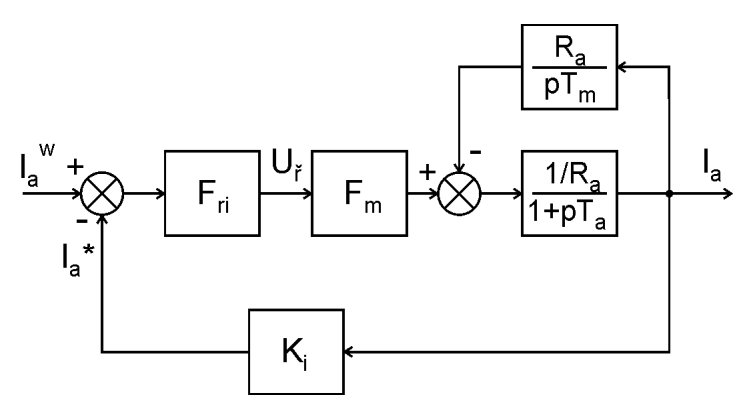
\includegraphics[width=1\linewidth]{ProudovaRegulace.png}
    \caption{Blokové schéma podřazené proudové regulace}
    \label{fig:ProudovaRegulace}
\end{figure}

\begin{figure}[H]
    \centering
    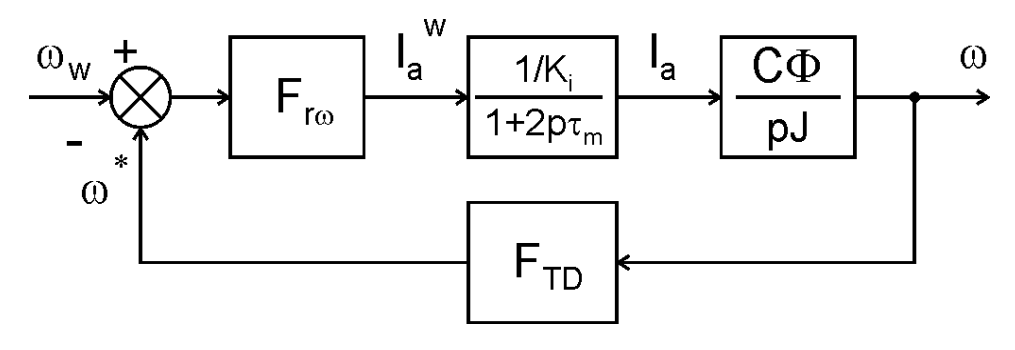
\includegraphics[width=1\linewidth]{OtackovaRegulace.png}
    \caption{Blokové schéma nadřazené otáčkové regulace}
    \label{fig:OtackovaRegulace}
\end{figure}

\begin{figure}[H]
    \centering
    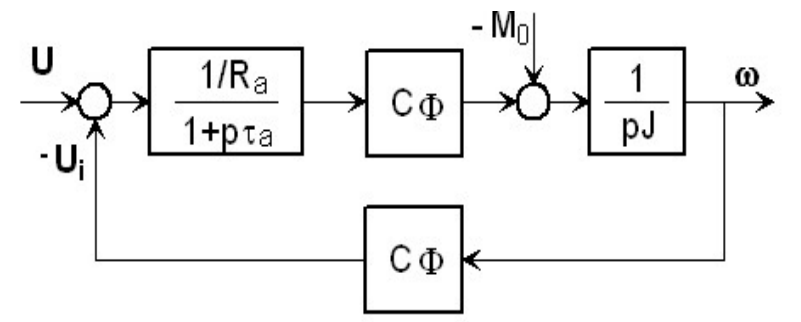
\includegraphics[width=1\linewidth]{ModelSSmotoru.png}
    \caption{Matematický model stejnosměrného motoru}
    \label{fig:ModelSSmotoru}
\end{figure}

\begin{figure}[H]
    \centering
    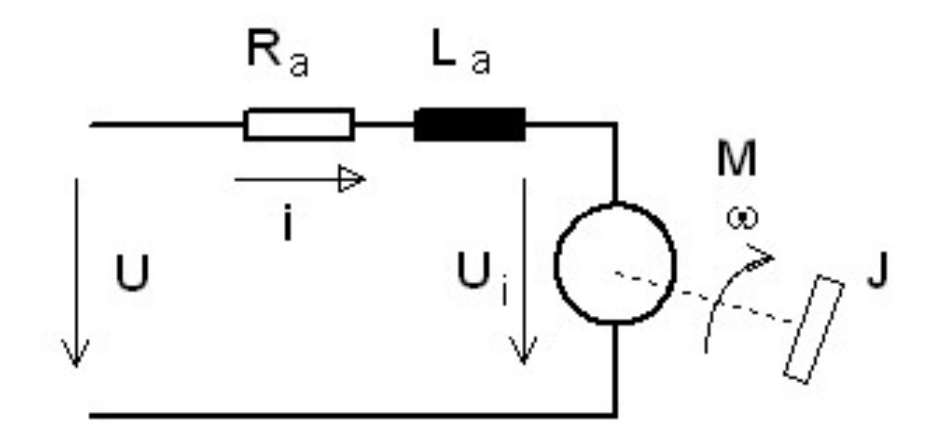
\includegraphics[width=1\linewidth]{ElektrickyModelSSmotoru.png}
    \caption{Elektrický model stejnosměrného motoru}
    \label{fig:ElektrickyModelSSmotoru}
\end{figure}

\section{Odvození konstant motoru}
\subsection{Odvození elektromagnetické časové konstanty}

Cílem této kapitoly je odvodit konstantu motoru $C\Phi{}$, elektromagnetickou časovou konstantu $\tau{}a$ a odpor vinutí $R_a$. 

Motor byl mechanicky zablokován. Na motor jsme nastavili požadovanou hodnotu napětí $2V$ při frekvenci $f = 0.2Hz$ a následně se na počítači sledovala odezva motoru naměřená pomocí měřící karty.

Proud na motoru se ustálil na $Ia = 12A$ při $2V$. 

Dále jsme ještě pomocí voltmetru změřili napětí na samotném motoru a to je $Ua = 1,42V$. Napětí je menší než jsme stanovili v programu kvůli tomu, že obvod při tak nízkém nastaveném napětí (a tedy i rychlosti) má velmi malou účinnost kvůli různým ztrátám na motoru. Dá se předpokládat, že pokud by napětí bylo třeba jmenovitých $30V$, pak by ztráty procentuálně nebyly tak velké.

Z toho je možné si dopočítat odpor motoru, který činí $R_a = 118,3 m\Omega$

\begin{equation}
    R_a = \frac{U_a}{I_a} = \frac{1,42V}{12A} = 118,3m\Omega
    \label{eq:VypocetOdporuMotoru}
\end{equation}

Z měřící karty v počítači jsme dostali tyhle data o průběhu proudu na motoru a jsou na grafu \ref{fig:proudovaExponenciala}.
\begin{figure}[H]
    \centering
    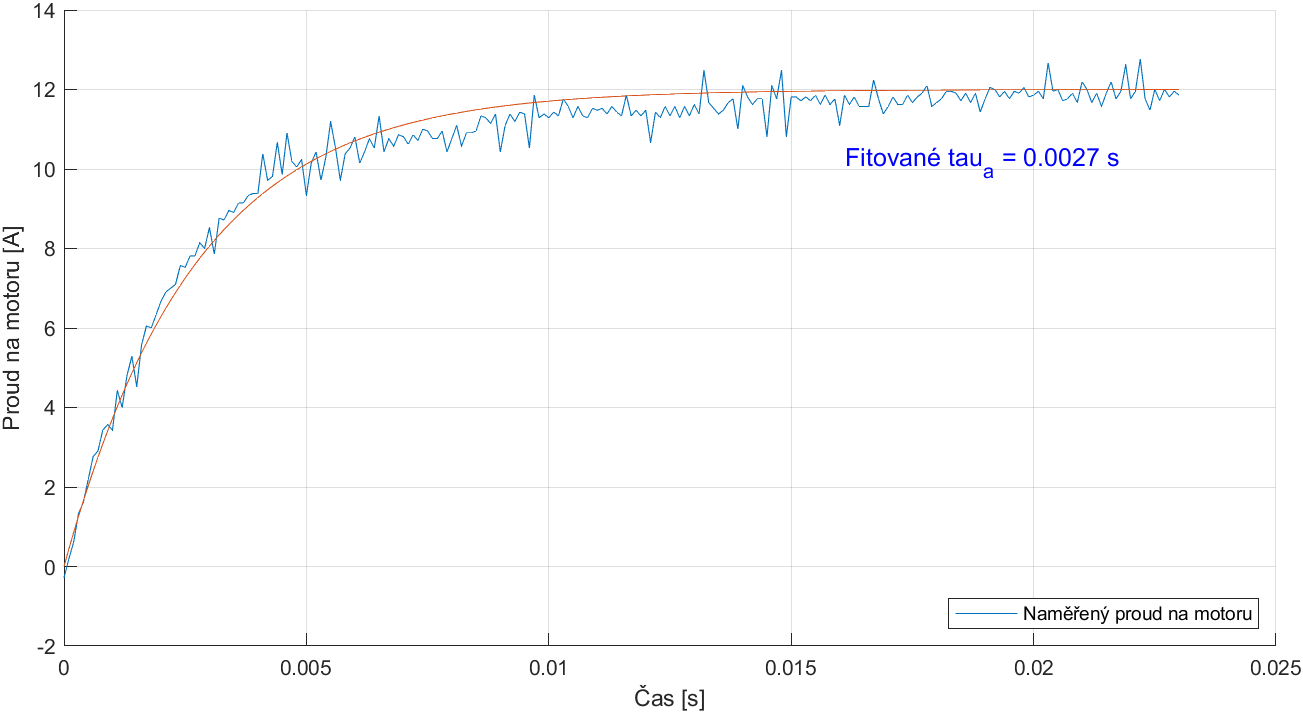
\includegraphics[width=1\linewidth]{proudovaExponenciala.png}
    \caption{Závislost proudu na čase při zablokovaném motoru}
    \label{fig:proudovaExponenciala}
\end{figure}

Průběh proudu motorem je tedy exponenciální. V grafu byl useknutý časový úsek kdy exponenciála ještě nezačínala a to nám umožnilo nafitovat do dat fitovací funkci $I = 12*(1-e^{-t/\tau{}})$ kde jsme z fitování získali časovou konstantu motoru $\tau_a = 2,7 ms$.

\subsection{Odvození konstanty stroje $C\Phi{}$}
Z matematického popisu motoru \ref{fig:ModelSSmotoru} víme že je napětí na motoru popsáno vztahem:

\begin{equation}
    u_a = R_ai_a + L_a\frac{di}{dt} + c\phi\omega
    \label{eq:RovniceMotoru}
\end{equation}

Pokud budeme uvažovat motor v ustáleném stavu pak bude změna proudu nulová a tak vypadne člen s indukčností motoru $L_a$. Poté bude rovnice pro výpočet konstanty stroje:

\begin{equation}
    C\Phi{} = \frac{U_a-R_aI_a}{\omega} = \frac{9,7 - 118,3\cdot{10^{-3}}\cdot{}1,8}{138} = 0.069Vs
    \label{eq:VypocetCPhiStroje}
\end{equation}

\section{Výpočet regulátoru pro metodu OM}
Pro návrh regulátoru metodou OM je potřebné si ještě určit časovou konstantu měniče která vychází z periody PWM - protože ten do soustavy také vnáší zpoždění.

\begin{equation}
    \tau_m = 1,5\cdot{}T_{pwm} = 1,5\cdot{}50\mu{}s = 75\mu{}ms
    \label{eq:VypocetCasoveKonstantyMotoru}
\end{equation}

V soustavě pro kterou navrhujeme regulátor máme tedy dvě časové konstanty: $\tau_a = 2,7 ms$ a $\tau_m = 75\mu{}s$ a tak regulátor navrhneme tak, aby eliminoval elektromechanickou časovou konstantu motoru. Takže $\tau_a = \tau_{\sigma}$.

Nyní je možné si vypočítat koeficienty metody OM. Vyházíme z rovnice:
\begin{equation}
    F_{RI} = F_{OM}\cdot\frac{1}{F_S}
\end{equation}
\begin{equation}
    \text{kde je přenos soustavy} F_S = \frac{1/R_a}{(1 + p\tau_m)\cdot{}(1+p\tau_a)}
\end{equation}
\begin{equation}
    F_{RI}(p) = \frac{R_a\cdot{}(1+p\tau_a)}{2\tau_mp} = \frac{R_a}{2\tau_mp} + \frac{R_a\tau_a}{2\tau_m} = I\cdot{}\frac{1}{p} + P
\end{equation}
Z těchto výpočtů lze vidět jak se počítají koeficienty $I$ a $P$ což jsou zesílení složek PI regulátoru.
\begin{itemize}
    \item $I_{slozka} = \frac{118,3\cdot{}10^{-3}}{2\cdot{}75\cdot{}10^{-6}} = 788,7$
    \item $P_{slozka} = \frac{118,3\cdot{}10^{-3}\cdot{}2,7\cdot{}10^{-3}}{2\cdot{}75\cdot{}10^{-6}} = 2,1294$
\end{itemize}

Výsledná rovnice PI regulátoru je tedy:
\begin{equation}
    F_{RI}(p) = 788,7\cdot{}\frac{1}{p} + 2,1294
\end{equation}

\subsection{Důsledek PI regulátoru navrženého dle metody OM}

Pro otestování funkčnosti PI regulátoru lze nastavit na motor stejné napětí, a zase se dá sledovat jaký bude motor reagovat.

Zde je znovu průběh motoru exponenciální a tak je možné nafitovat exponenciálu abychom dostali časovou konstantu, stejně jako v předešlém případě. Rovnice fitované exponenciály je v tomto případě $I = 10*(1-e^{-t/\tau{}})$ protože proud se ustálil na $10A$ a z této rovnice vyšla nová časová konstanta obvodu $\tau = 0.2ms$, což je asi 13x rychlejší odezva motoru. Tato odezva je zobrazena na grafu \ref{fig:DusledekPIRegulatoru}.

Tahle rychlost se tam ale neobjevila jenom tak. Byla způsobena tím, že proudový regulátor na motor nastavil mnohem větší napětí než bylo nastavené předtím. Napětí vzrostlo až na hodnotu $15.24V$ hned na začátku měření. Tohle dává smysl, jelikož napětí na indukčnosti je větší čím rychlejší je změna proudu.

Při používání proudového regulátoru se tedy musí dát pozor, že je napětí dostatečné aby pokrylo napěťové požadavky, které proudový regulátor požaduje, anebo alespoň aby bylo napětí saturované na maximální přípustné hodnotě. 

\begin{figure}[H]
    \centering
    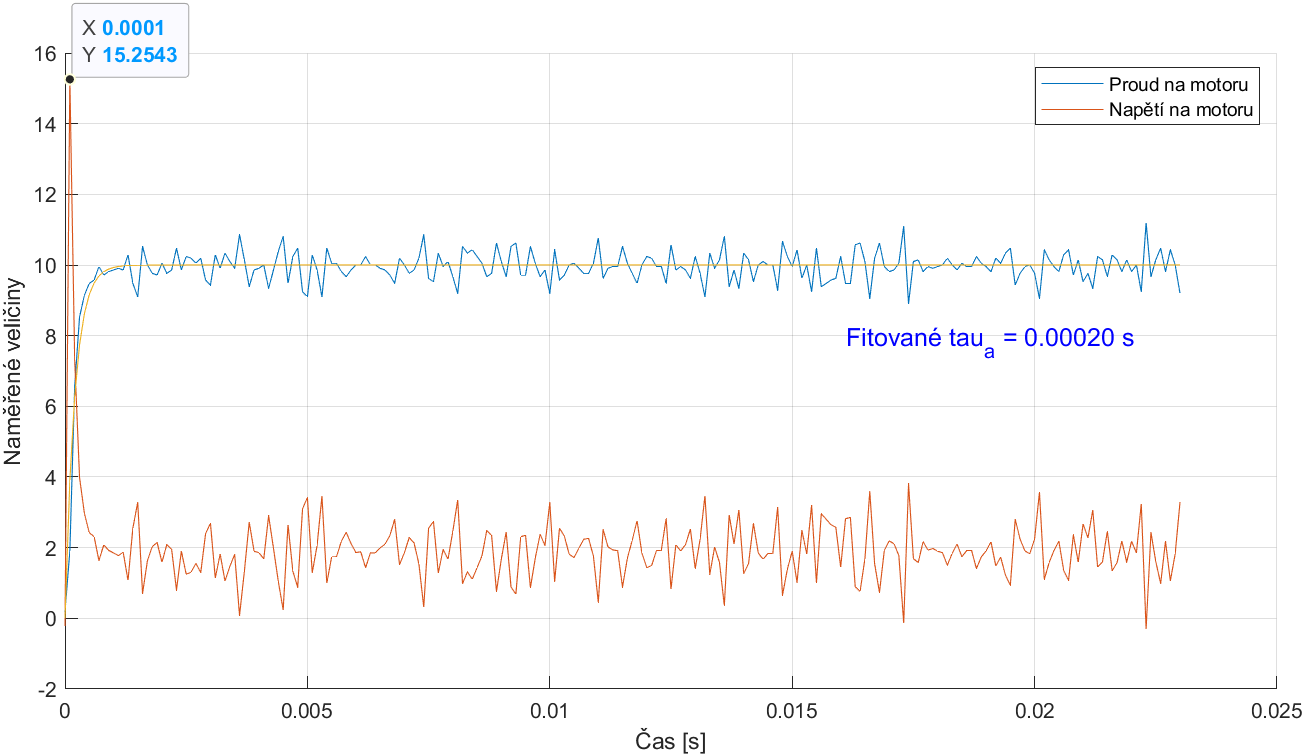
\includegraphics[width=1\linewidth]{DusledekPIRegulatoru.png}
    \caption{Nastavení stejného napětí na motor $2V$ s PI regulátorem}
    \label{fig:DusledekPIRegulatoru}
\end{figure}

\section{Identifikace momentu setrvačnosti}

Dalším úkolem v rámci tohoto laboratorního měření bylo identifikovat moment setrvačnosti aby bylo možné sestavit regulátor otáček.

Vycházíme z mechanického popisu rovnice stejnosměrného motoru (v rovnici zanedbáváme tření):

\begin{equation}
    M = J\frac{d\omega}{dt}+c\phi{}i
    \label{eq:MechanickaRovniceMotoru}
\end{equation}

Moment setrvačnosti se tak dá změřit tím, že si nastavíme na motor nějaký proud (v našem případě 5A) při kterém bude motor zrychlovat na maximální hodnotu po trase rampy. Díky tomu budeme znát $\Delta{}\omega/\Delta{}t$, konstantu stroje i proud. Pokud stroj pojede naprázdno tak bude navíc výsledný M rovný nule, takže můžeme řešit pouze pravou stranu rovnice \ref{eq:MechanickaRovniceMotoru}. Data pro výpočet momentu setrvačnosti jsou zobrazené na grafu \ref{fig:VypocetMomentuSetrvacnostiMotoru}.

\begin{figure}[H]
    \centering
    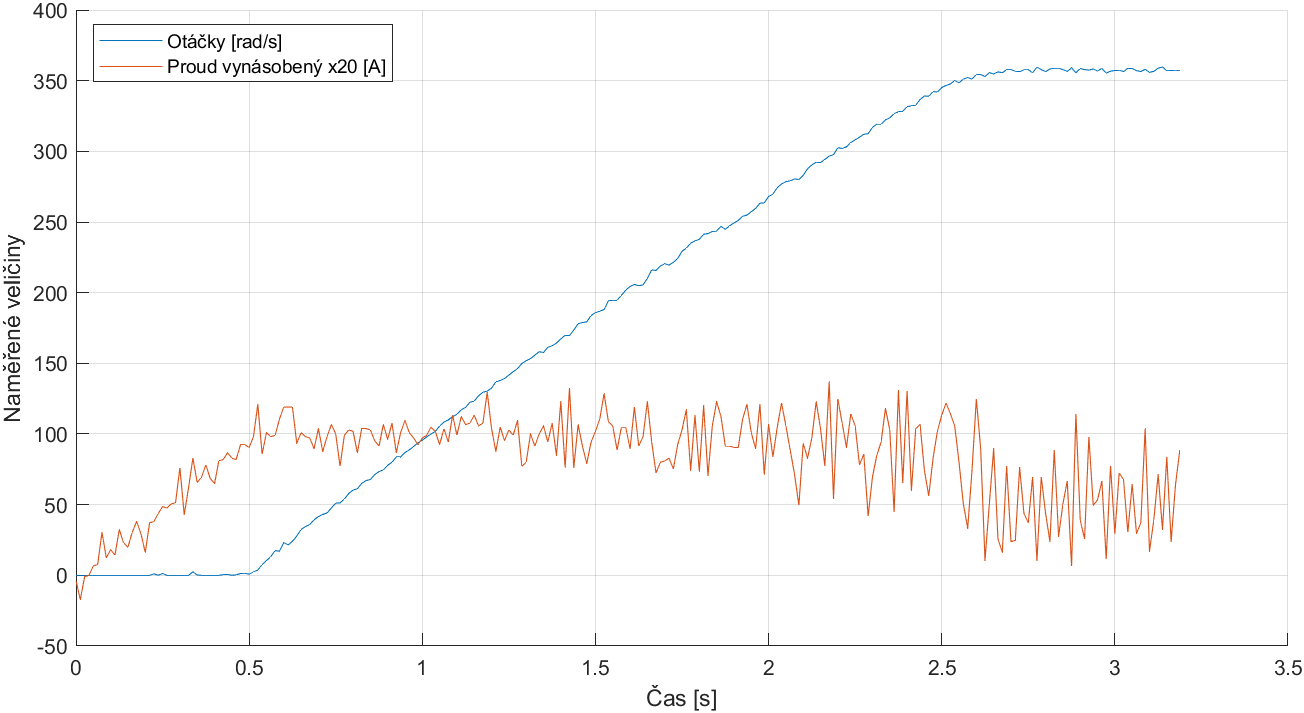
\includegraphics[width=1\linewidth]{VypocetMomentuSetrvacnostiMotoru.png}
    \caption{Graf pro výpočet momentu setrvačnosti motoru}
    \label{fig:VypocetMomentuSetrvacnostiMotoru}
\end{figure}

Celkový proud co vytváří moment společně s konstantou není rovný požadovaných $5A$, protože se vždy bude část momentu využívat na pokrytí statického momentu. To jsme naměřili, že je $1,8A$. Pro výpočet úhlového zrychlení jsme si zvolili dva body. První bod je [$1s$; $95,6rad/s$] a druhý bod je [$2,5s$; $345rad/s$].

\begin{equation}
    J = \frac{\Delta{t}\cdot{}c\phi{}I}{\Delta{\omega}} = \frac{(2,5 - 1)\cdot{}0.069\cdot{}(5-1.8)}{(345 - 95,6)} = 1.3\cdot{}10^{-3}kgm^2
    \label{eq:VypocetMomentSetrvacnostiMotoru}
\end{equation}

\section{Ukázka regulátoru otáček}

V tomto laboratorním cvičení jsme si také ukázali jaký efekt bude mít, když na tuto soustavu ještě nasadíme nadřazený regulátor otáček. Tento regulátor způsobí, že můžeme zadávat otáčky jako vstup do soustavy. Chyba v otáčkách se převede do proudu a ten je vstupem do proudového regulátoru, který řídí motor. Jde tedy o kaskádní regulaci. Důvodem proč navrhnout otáčkový regulátor je, že udržuje otáčky na chtěné hodnotě a tedy pokud se zvýší moment na hřídeli, regulátor zvýší proud a tím si motor udrží otáčky.

Odezva motoru při regulování na 100 radiánů za sekundu je na grafu \ref{fig:OdezvaNaOtackovyRegulator}.

\begin{figure}[H]
    \centering
    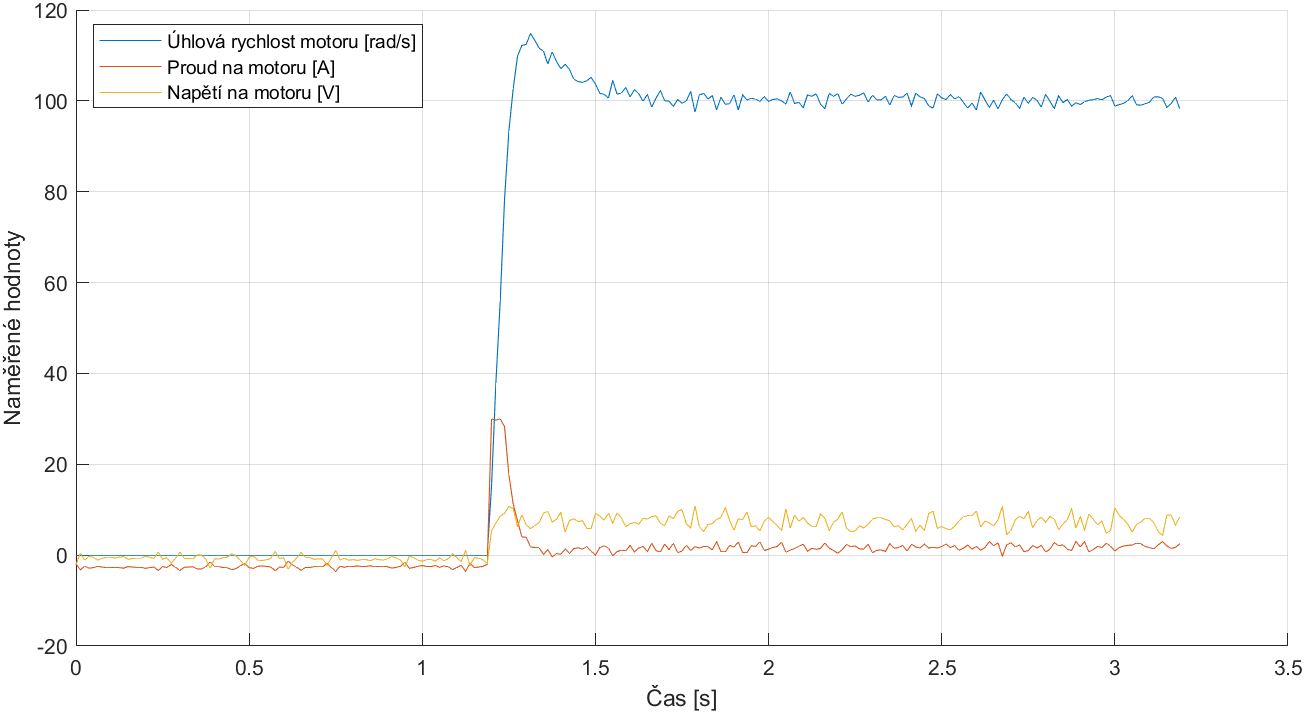
\includegraphics[width=1\linewidth]{OdezvaNaOtackovyRegulator.png}
    \caption{Odezva systému na otáčkový regulátor se vstupem $100 rad/s$}
    \label{fig:OdezvaNaOtackovyRegulator}
\end{figure}

\section{Závěr}

V rámci provedeného experimentu byly stanoveny konstanty stejnosměrného motoru. Byl určen odpor vinutí $R_a$ s hodnotou $118,3 \, m\Omega$ a elektromagnetická časová konstanta $\tau_a$ s hodnotou $2,7 \, ms$. Dále byla vypočtena konstanta stroje $C\Phi{}$ s hodnotou $0.069 \, Vs$. Tyto parametry jsou nezbytné pro návrh a implementaci řídicích algoritmů, jelikož popisují dynamické charakteristiky motoru a jeho odezvu na elektrické signály. Moment setrvačnosti $J$ byl identifikován jako $1.3 \cdot 10^{-3} \, kgm^2$, což je důležité pro návrh regulace otáček motoru.

Protokol dokumentoval průběh experimentu. Teoretická část objasnila princip kaskádní regulace stejnosměrného motoru s podřazenou proudovou a nadřazenou otáčkovou smyčkou. Kapitola o postupu měření popsala metody použité pro identifikaci parametrů stroje. Následovalo zpracování dat, zahrnující výpočty konstant motoru z naměřených veličin a aproximaci exponenciální funkcí pro určení časové konstanty.

V experimentu se vyskytly dílčí odchylky, například nižší hodnota naměřeného napětí na motoru v zablokovaném stavu, pravděpodobně v důsledku ztrát při nízkých úrovních napětí. Návrh regulátoru metodou optimálního modulu (OM) rovněž vycházel z určitých idealizací, jako je zanedbání deadtimu měniče. Tyto faktory mohly potenciálně ovlivnit přesnost stanovených parametrů a návrhu regulátoru. Nicméně, získané výsledky poskytují náhled způsob návrhu regulace která funguje, protože po navržení proudové regulace se dosáhne motor požadované hodnoty proudu cca 13x rychleji.

Realizovaný experiment přispěl k hlubšímu porozumění chování stejnosměrného motoru a principům návrhu jeho regulace. Identifikace parametrů motoru a ověření účinnosti proudového regulátoru navrženého metodou OM demonstrovaly jak je možné regulovat proud DC motoru na základě matematických modelů. Implementace nadřazené regulace otáček prokázala schopnost přesného řízení otáček i při rostoucím momentu. Získané poznatky mají význam pro další studium v oblasti elektrických pohonů a pro potenciální praktické aplikace vyžadující precizní řízení stejnosměrných motorů.

\end{document}